\documentclass[aspectratio=169,11pt]{beamer}
\usepackage[T1]{fontenc}
\usepackage{lmodern,tikz,booktabs,graphicx,hyperref}
\usepackage{media9}
\usetikzlibrary{arrows.meta,positioning,shapes.geometric}
\definecolor{navy}{HTML}{0B2545}\definecolor{teal}{HTML}{13A89E}\definecolor{amber}{HTML}{F2A541}\definecolor{soft}{HTML}{EEF3F8}
\usetheme{default}
\setbeamercolor{frametitle}{fg=white,bg=navy}
\setbeamercolor{normal text}{fg=navy}
\setbeamercolor{block title}{bg=teal,fg=white}\setbeamercolor{block body}{bg=soft,fg=navy}
\setbeamertemplate{navigation symbols}{}
\setbeamerfont{frametitle}{series=\bfseries,size=\Large}
\setbeamertemplate{frametitle}{\nointerlineskip
 \begin{tikzpicture}[remember picture,overlay]
 \fill[navy] (current page.north west) rectangle ([yshift=-1.1cm]current page.north east);
 \fill[teal] ([yshift=-1.1cm]current page.north west) rectangle ([yshift=-1.18cm]current page.north east);
 \node[anchor=west,text=white,font=\Large\bfseries] at ([xshift=.8cm,yshift=-.55cm]current page.north west) {\insertframetitle};
 \end{tikzpicture}\vspace{.6cm}}
\setbeamertemplate{footline}{\hfill\scriptsize\color{navy!60}AutoFOAM \,|\, SimuNetics \,|\, \insertframenumber/4\hspace{.6cm}\vspace{.3cm}}
\newcommand{\kpi}[2]{\begin{tikzpicture}\node[fill=soft,draw=teal,rounded corners=4pt,minimum width=2.9cm,minimum height=1.3cm,align=center]{{\Large\bfseries\color{teal}#1}\\[-1pt]{\scriptsize #2}};\end{tikzpicture}}
\tikzset{st/.style={draw=navy,fill=soft,rounded corners=3pt,minimum width=1.75cm,minimum height=.95cm,align=center,font=\scriptsize},
 ar/.style={-{Stealth},thick,teal}}
\begin{document}

\begin{frame}{From a sentence to a converged CFD case -- automatically}
\begin{columns}[T]
\column{.5\textwidth}
\begin{block}{The problem}
\small OpenFOAM is powerful and free, but each case needs a dozen interlinked dictionaries, a mesh and the right solver. Setup is slow, error-prone and needs scarce expertise.
\end{block}
\begin{block}{AutoFOAM}
\small A self-improving AI agent (fine-tuned 14B model) that turns a plain-English request into a meshed, configured, \emph{running} OpenFOAM v2412 simulation.
\end{block}
\vspace{2pt}\small\textit{``NACA0012 airfoil, AoA 5$^\circ$, Re=$10^6$, chord=1\,m''}
\column{.5\textwidth}
\centering
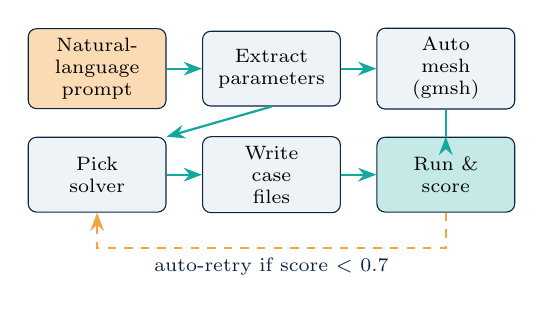
\begin{tikzpicture}[node distance=.35cm and .45cm]
\node[st,fill=amber!40](a){Natural-\\language\\prompt};
\node[st,right=of a](b){Extract\\parameters};
\node[st,right=of b](c){Auto\\mesh\\(gmsh)};
\node[st,below=of a](d){Pick\\solver};
\node[st,right=of d](e){Write\\case\\files};
\node[st,right=of e,fill=teal!25](f){Run \&\\score};
\draw[ar](a)--(b);\draw[ar](b)--(c);\draw[ar](c.south)--++(0,-.0)|-(c.south|-f.north)--(f.north);
\draw[ar](d)--(e);\draw[ar](e)--(f);
\draw[ar](b.south)--(d.north east);
\draw[ar,amber,dashed](f.south)--++(0,-.45)-|node[pos=.25,below,font=\scriptsize,text=navy]{auto-retry if score $<$ 0.7}(d.south);
\end{tikzpicture}

\vspace{.4cm}
\begin{minipage}{.95\linewidth}\small
$\bullet$ 7 solver families, 13 mesh templates\\
$\bullet$ Runs on-premise: your data stays with you\\
$\bullet$ No manual CAD or case editing
\end{minipage}
\end{columns}
\end{frame}

\begin{frame}{Proven results: reliable, autonomous, out-of-distribution}
\centering\footnotesize
\begin{tabular}{@{}c@{\hspace{.15cm}}c@{\hspace{.15cm}}c@{\hspace{.15cm}}c@{}}
& \textbf{NACA airfoil} & \textbf{Cylinder cross-flow} & \textbf{S-bend duct}\\
\raisebox{.9cm}{\rotatebox{90}{Mesh}} & 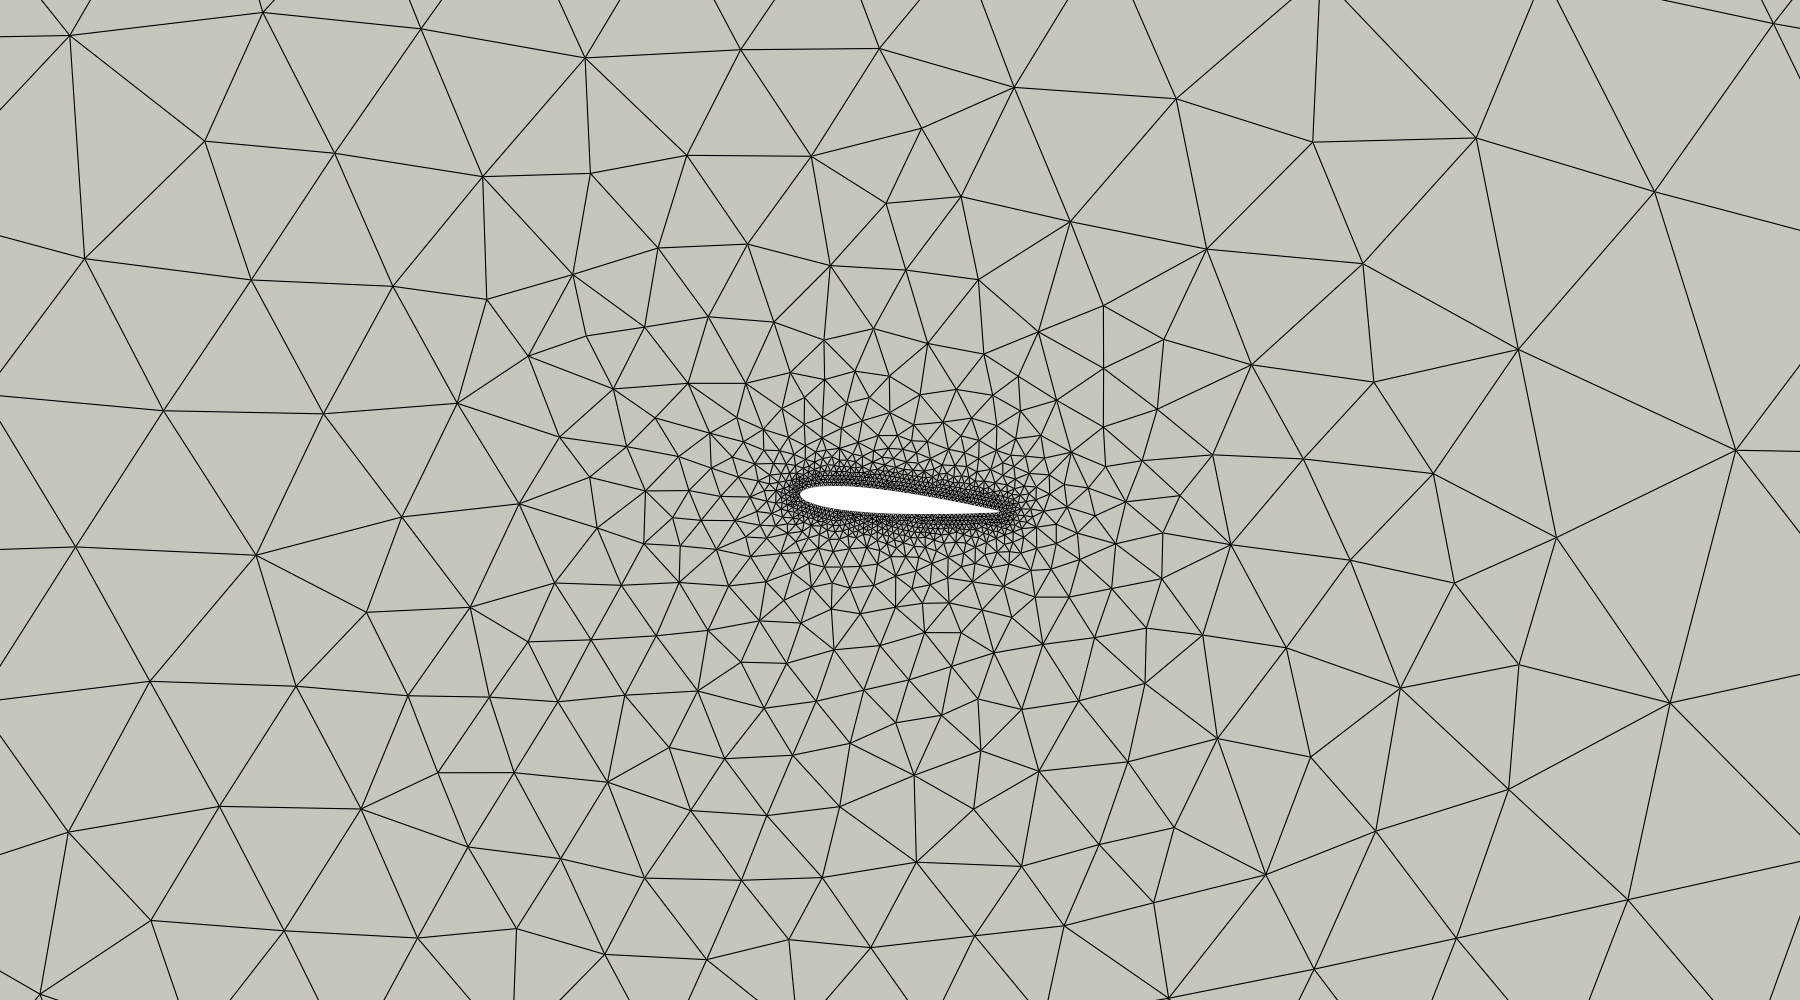
\includegraphics[height=1.8cm]{figures/airfoil_mesh_zoom_wide.png} & 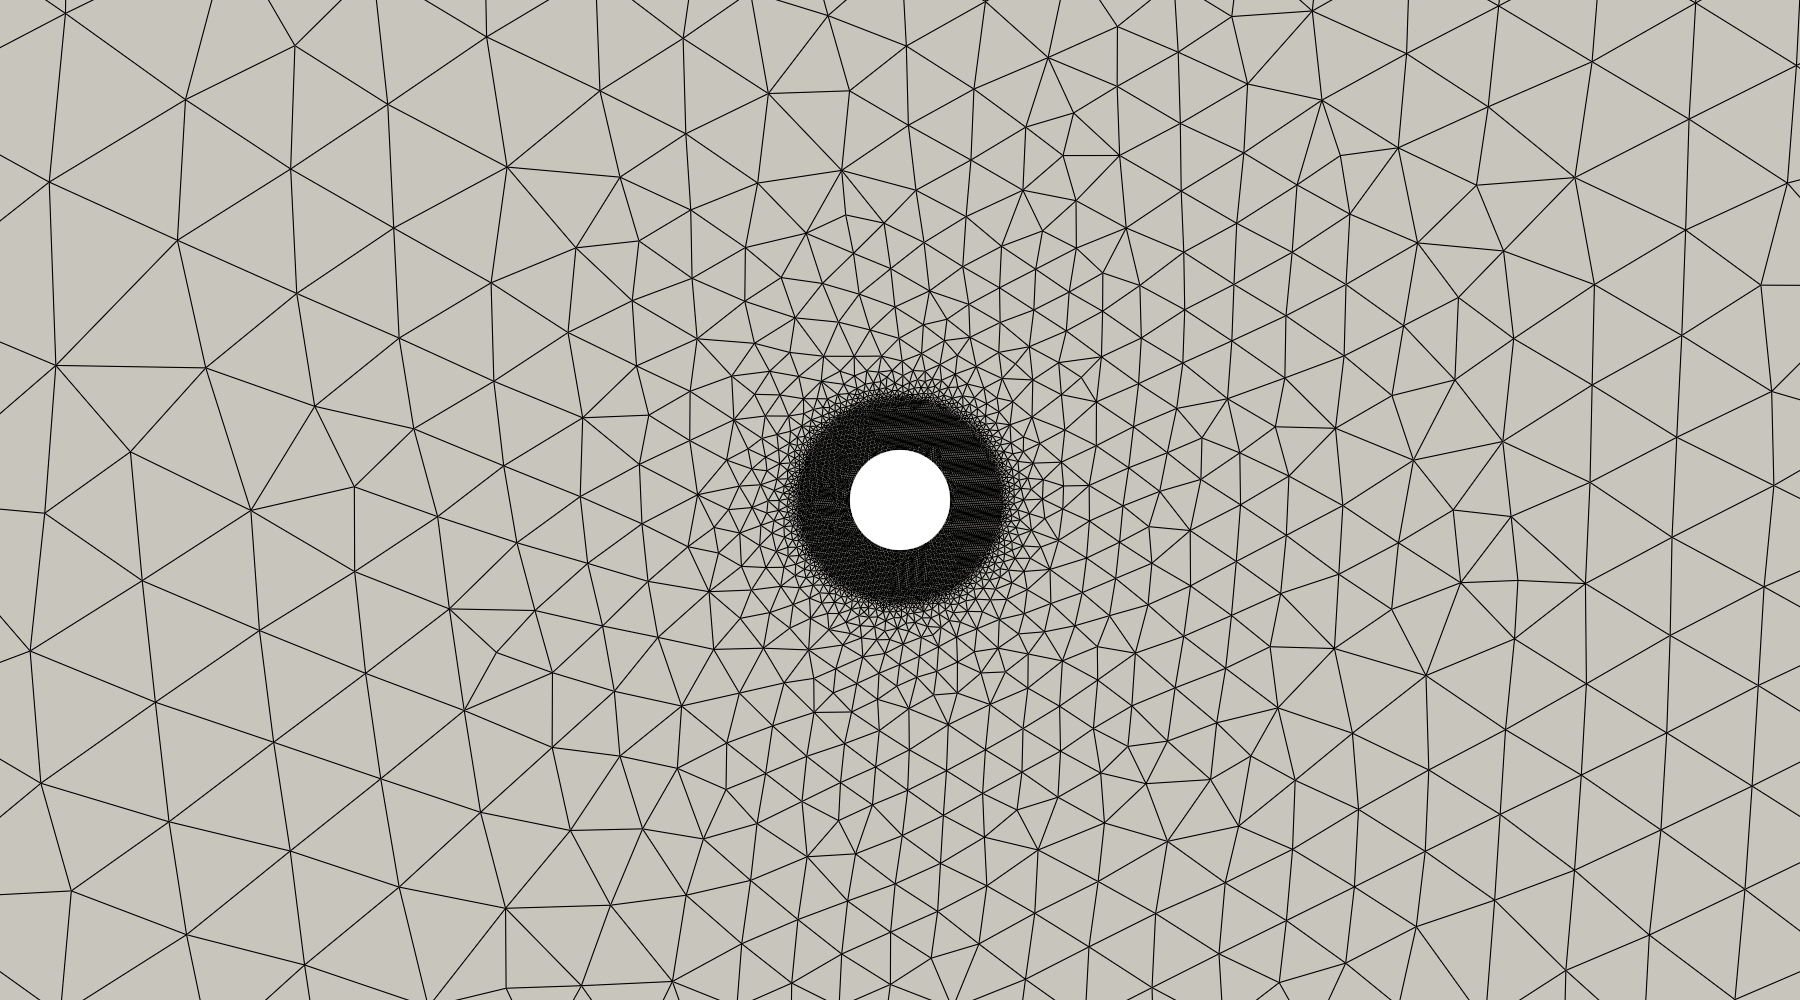
\includegraphics[height=1.8cm]{figures/cylinder_mesh_zoom.png} & 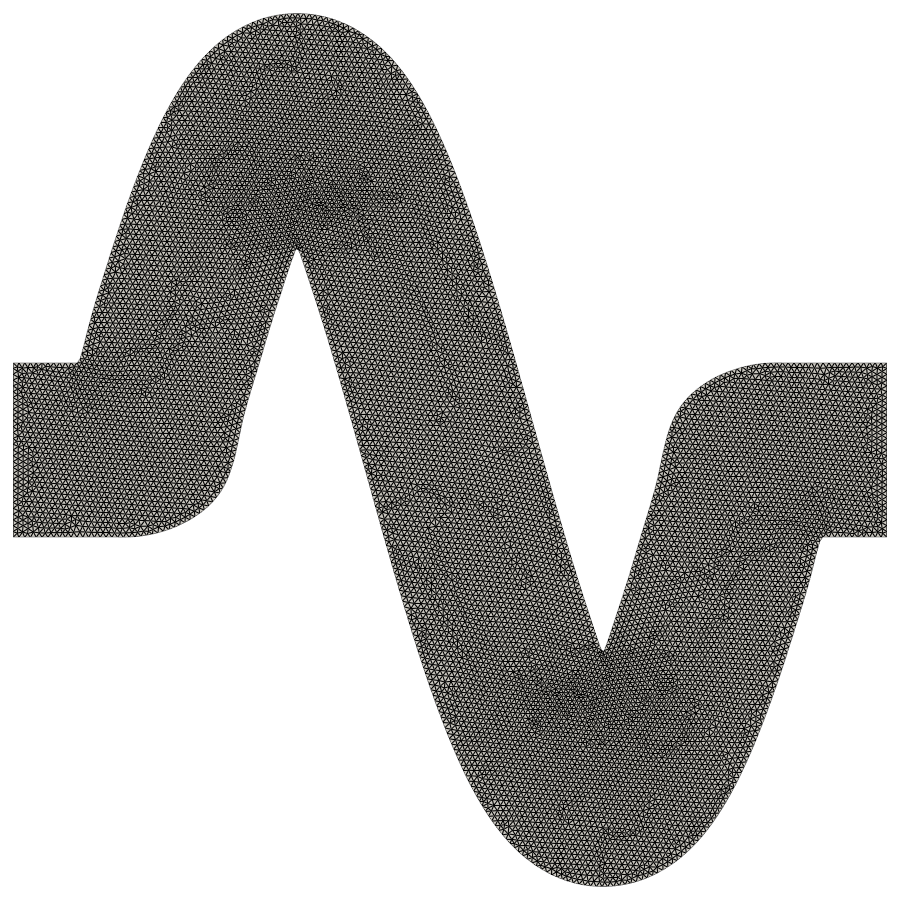
\includegraphics[height=1.8cm]{figures/clean_sbend_mesh.png}\\
\raisebox{.8cm}{\rotatebox{90}{Velocity}} & 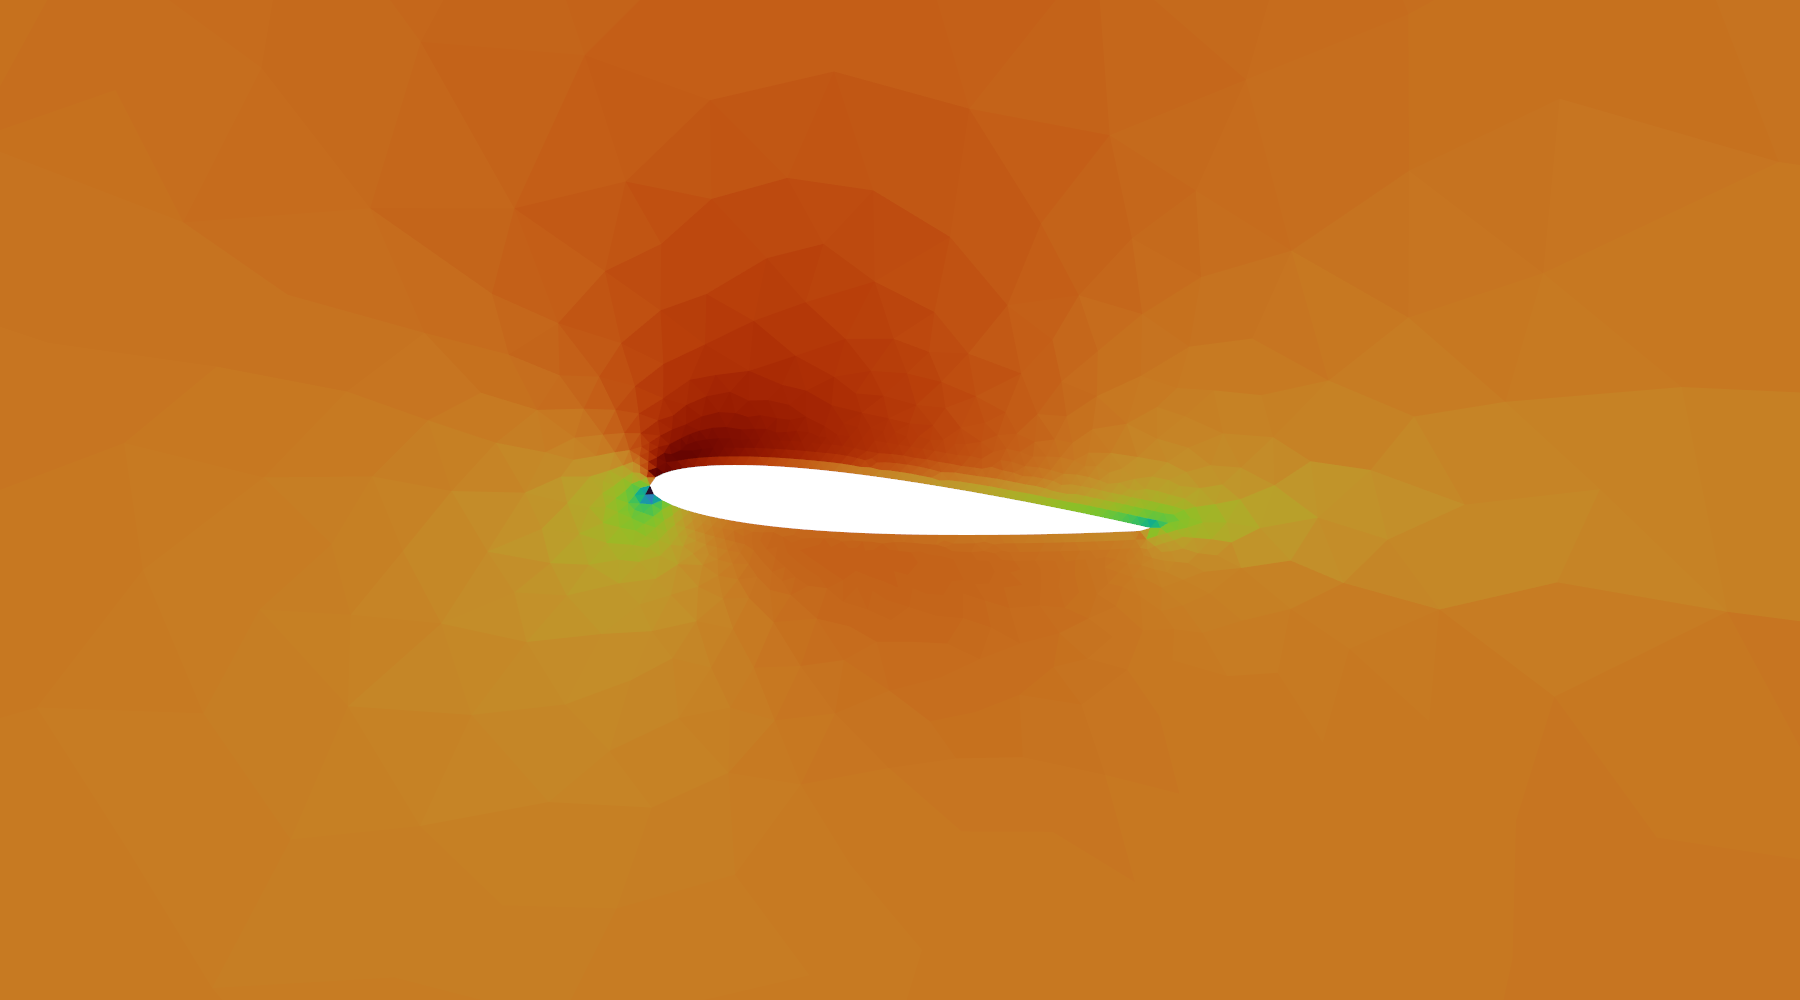
\includegraphics[height=1.8cm]{figures/airfoil_zoom_mid.png} & 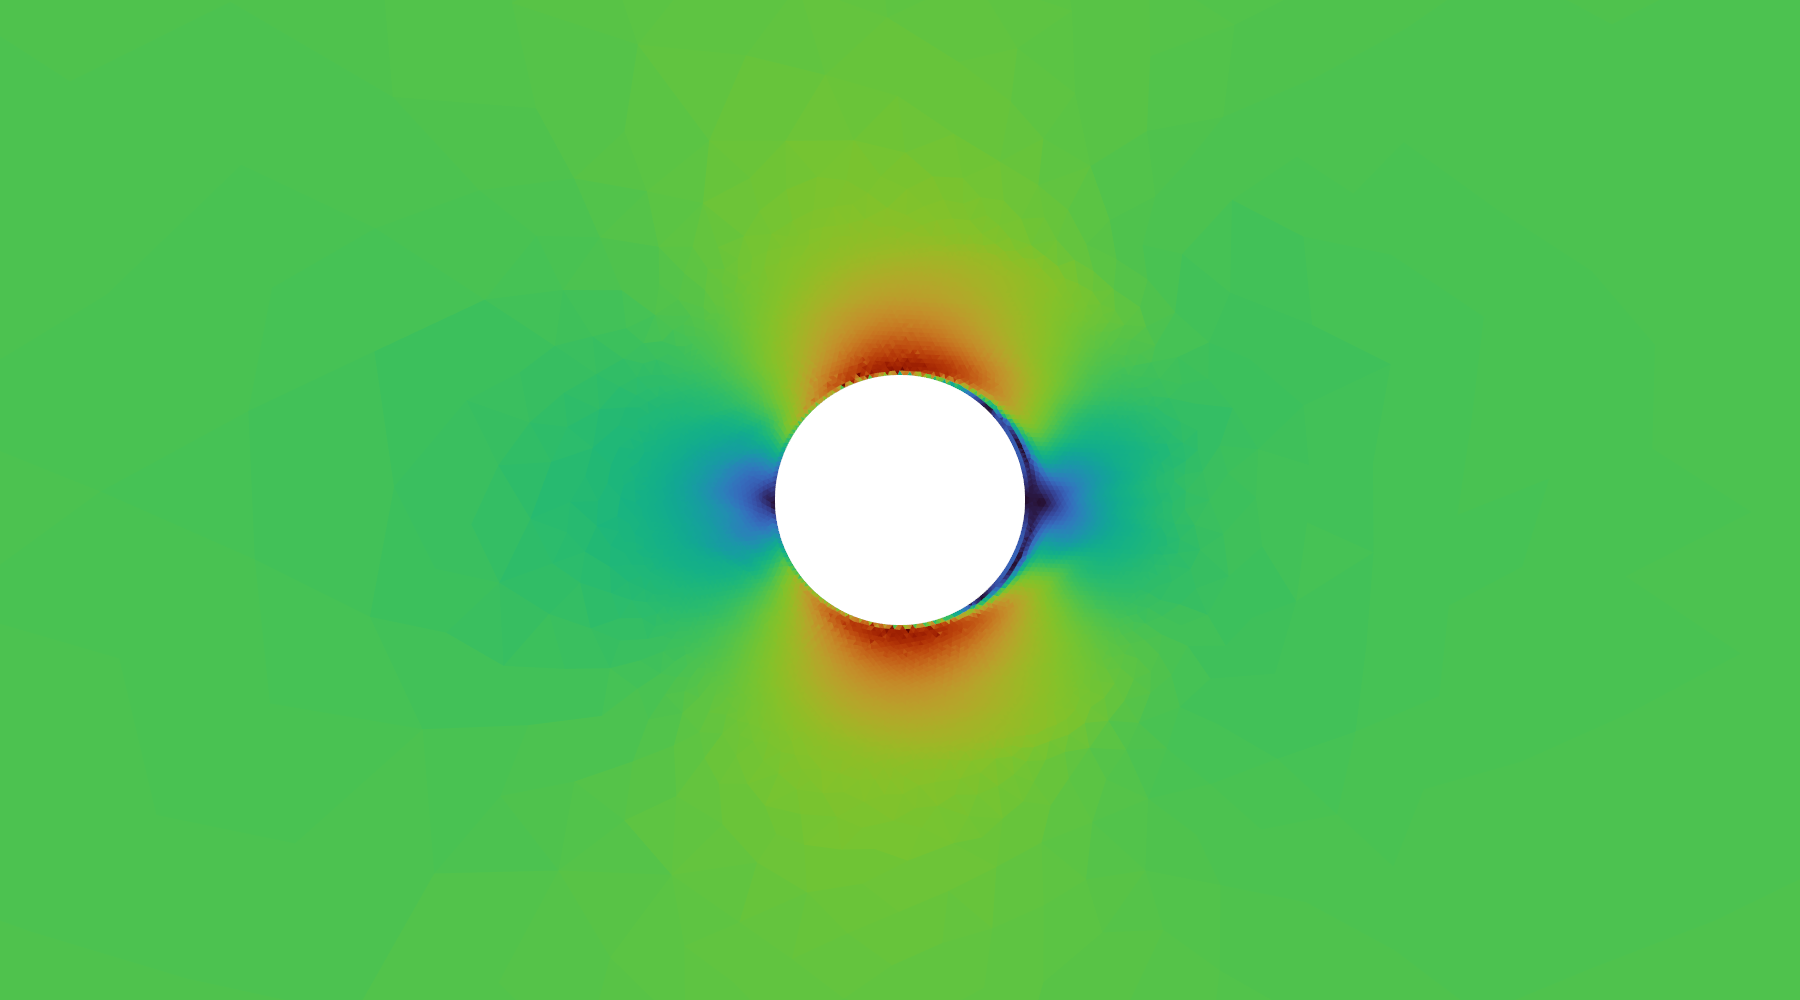
\includegraphics[height=1.8cm]{figures/cylinder_zoom_mid.png} & 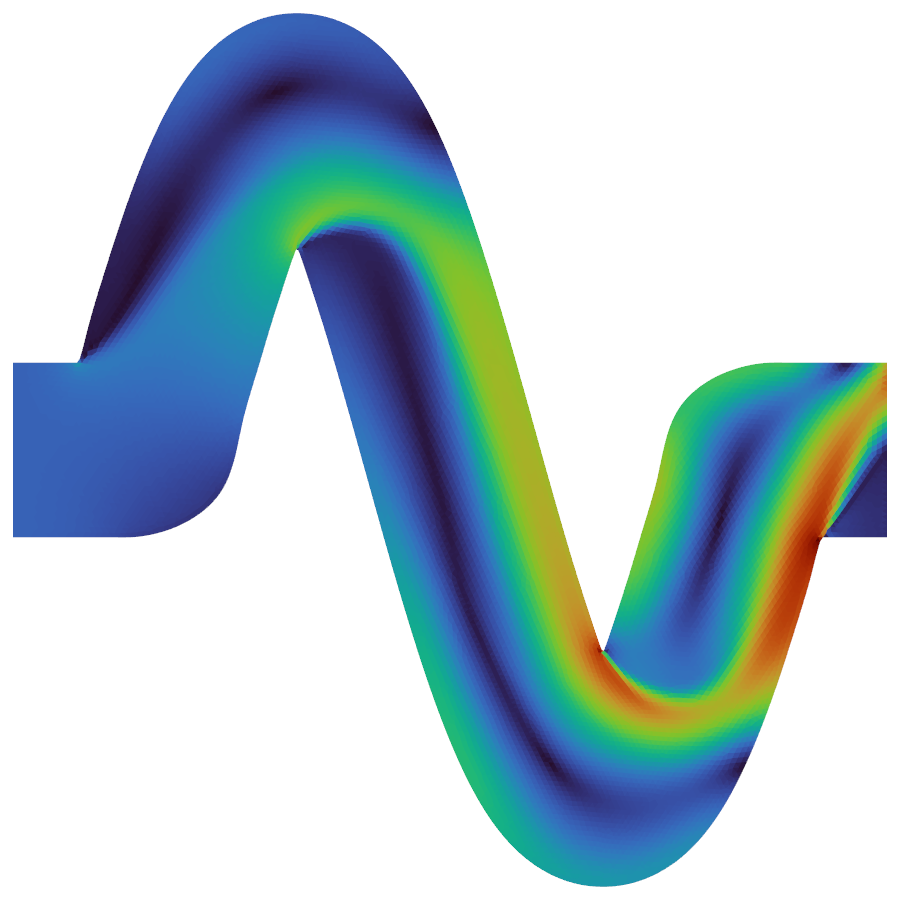
\includegraphics[height=1.8cm]{figures/clean_sbend_velocity.png}
\end{tabular}

\vspace{.2cm}
\kpi{110/110}{cases ran, no fatal error}%
\kpi{96.4\%}{correct solver (106/110)}%
\kpi{13/13}{mesh geometries}%
\kpi{7/7}{solver families}

\vspace{.1cm}{\scriptsize Held-out prompts, not seen in training. Each case above came from one prompt, zero manual steps.}
\end{frame}

\begin{frame}{Self Evolving AI}
\begin{columns}[T]
\column{.52\textwidth}
\begin{block}{Seven-layer self-evolution loop}
\scriptsize
\begin{tabular}{@{}rl@{}}
\textbf{1} & Self-correct failed runs from solver logs\\
\textbf{2} & Auto-curate only high-scoring cases\\
\textbf{3} & Fine-tune, then gate on held-out tests\\
\textbf{4} & Learn from fail$\to$fix pairs (DPO)\\
\textbf{5} & Anchor on original data: no forgetting\\
\textbf{6} & Target the weakest solver family\\
\textbf{7} & Regression check: no worse model ships
\end{tabular}
\end{block}
\small\textbf{Built-in safeguards:} retrieval from OpenFOAM tutorials, surgical dictionary fixes, prompt-diversity paraphrasing.
\vspace{4pt}
\begin{block}{Extensible}
\small This workflow can be extended to other CFD tools and to geometries of your choice.
\end{block}
\column{.46\textwidth}
\begin{block}{What you get}
\small
$\bullet$ Hours of setup cut to one prompt\\
$\bullet$ Standard OpenFOAM cases you can inspect and edit\\
$\bullet$ Python API, interactive REPL and batch runs\\
$\bullet$ Self-hosted: one GPU ($\ge$24\,GB) + OpenFOAM v2412
\end{block}
\begin{block}{Work with us}
\small
Pilots, custom solver/geometry extensions and commercial licensing .\\[2pt]
\scriptsize github.com/AGN000/AutoFOAM 
\end{block}
\end{columns}
\end{frame}
\begin{frame}{Live demo: AutoFOAM web interface}
\centering
\includemedia[width=.62\linewidth,height=.3488\linewidth,activate=pageopen,
 addresource=media/demo.mp4,
 flashvars={source=media/demo.mp4&autoPlay=false&loop=false},
 transparent,passcontext]{\includegraphics[width=.62\linewidth]{media/poster.png}}{VPlayer.swf}

{\scriptsize Click the video to play (Adobe Acrobat Reader). Other viewers: \href{run:media/demo.mp4}{open media/demo.mp4}.\\
Web UI: residual convergence, field contours and one-click ParaView.}
\end{frame}
\end{document}
